% Tipo de documento. En este caso es un art�culo, para folios A4, tama�o de la fuente 11pt y con p�gina separada para el t�tulo
\documentclass[a4paper,11pt,titlepage]{article}

% Carga de paquetes necesarios. OrdenesArticle es un paquete personalizado
\usepackage[spanish]{babel} 
\RequirePackage[T1]{fontenc}
\RequirePackage[ansinew]{inputenx} 
\usepackage[spanish,cap,cont,title]{OrdenesArticle}
\usepackage{array}
\usepackage{graphicx}
\usepackage{hyperref}
\usepackage{pifont}
\usepackage{listings}
\usepackage[usenames,dvipsnames]{color}
\usepackage{colortbl}
\usepackage{makeidx}
\hypersetup{bookmarksopen,bookmarksopenlevel=3,linktocpage,colorlinks,urlcolor=blue,citecolor=blue,
						linkcolor=blue,filecolor=blue,pdfnewwindow,
						pdftitle={Empresa a aduitar}, 
						pdfauthor={Juan Andrada, Jose Domingo L�pez, Antonio Mart�n Menor, Francisco Jos� Oteo}}


% Macro para definir una lista personalizada 
\newenvironment{milista}%
{\begin{list}{\textbullet}%
{\settowidth{\labelwidth}{\textbullet} \setlength{\leftmargin}{\dimexpr\labelsep+\labelwidth+5pt}
\setlength{\itemsep}{\dimexpr 0.5ex plus 0.25ex minus 0.25ex}
\setlength{\parsep}{\itemsep}
\setlength{\partopsep}{\itemsep}
\addtolength{\topsep}{-7.5pt}
}}%
{\end{list}}


\begin{document}

% En las p�ginas de portada e �ndices, no hay encabezado ni pie de p�gina
\pagestyle{empty} 

% Se incluye la portada
\begin{titlepage}
	\begin{center}
  	{\LARGE UNIVERSIDAD DE CASTILLA-LA MANCHA} \\
  	\bigskip
  	{\Large ESCUELA SUPERIOR DE INFORM�TICA} \\
  	\vspace{20mm}
  	
\includegraphics[scale=0.45, keepaspectratio]{esi_bw.png} \\
  	\vspace{20mm}
  	{\Huge \textbf{Definici�n de la empresa a auditar}} \\
  	\vspace{10mm}
  	{\LARGE \textsc{\textbf{DIGSOL: Soluciones Digitales a tu medida}}} \\
  	\vspace{30mm}
  	\today
  	\vspace{30mm}
  	\begin{flushleft}
  		{\large Juan Andrada Romero}\\
  		\vspace{1mm}
  		{\large Jose Domingo L�pez L�pez}\\
  		\vspace{1mm}
  		{\large Antonio Mart�n Menor de Santos}\\
  		\vspace{1mm}
  		{\large Francisco Jos� Oteo Fern�ndez}\\  		
  	\end{flushleft}
	\end{center}
\end{titlepage}

% Se ajusta la separaci�n entre p�rrafos
\parskip=10pt

% Aqui se incluyen los archivos .tex que forman el documento
\section{Definici�n de la empresa DIGSOL}

DIGSOL es una cadena espa�ola dedicada a la venta de diversos productos inform�ticos.

Sus or�genes se remontan al a�o 2000, cuando abri� su primera tienda en la capital
espa�ola. En los inicios, los productos que ofrec�a la tienda se reduc�an a ordenadores de
sobremesa, impresoras y diversos perif�ricos.

Poco a poco y gracias al empe�o de sus fundadores de ofrecer m�s y m�s productos
inform�ticos a los aficionados a las nuevas tecnolog�as, DIGSOL fue incorporando m�s productos a
su cat�logo tales como videoconsolas, tel�fonos m�viles, dispositivos de redes y c�maras digitales.

Paralelamente a este aumento en la variedad de los productos, se produce un incremento
tambi�n en el n�mero de tiendas repartidas por las principales ciudades espa�olas, alcanzando la
docena en torno al a�o 2003.

A mediados del 2004, la cadena crea DIGSOL LOW, una l�nea de productos de bajo
precio. El objetivo de esta gama de productos es que el cliente pague s�lo lo m�nimo, sin renunciar
a la calidad. Esta l�nea de productos tuvo una buena acogida por el p�blico y en el 2006 aparece la
l�nea DIGSOL LOW06, su sucesora, apostando fuertemente por la telefon�a m�vil.

Durante todo este tiempo la empresa sigue aumentando su n�mero de tiendas por el pa�s y
se abre camino en Portugal. Actualmente cuenta con 40 tiendas distribuidas por ambos pa�ses, y se
sit�a entre las 20 con m�s volumen de ventas del sector.

Fiel a sus or�genes, la empresa contin�a apostando por un trato personal de calidad,
destac�ndose en una de las impulsoras en la disposici�n de servicio t�cnico 24 horas para sus
clientes y la posibilidad de registrarse como cliente VIP de la cadena, accediendo de esta forma a
importantes ofertas y descuentos en todos los productos.

A partir de mediados de 2008, tras un per�odo de discreto crecimiento econ�mico y las
numerosas peticiones de soluciones inform�ticas por parte de cada vez m�s clientes, la compa��a
centra sus esfuerzos en consolidar la expansi�n nacional y abrir las puertas al mercado europeo.

Estas peticiones se alzan a favor de nuevas aplicaciones web que acerquen la cadena a un
mayor n�mero de usuarios y faciliten las gestiones v�a Internet. Por ello, la empresa ha desarrollado un sistema que 
que permite la realizaci�n de pedidos on-line, asoci�ndose a una empresa de transportes para poder distribuir los pedidos que se realizan en la Web con la mayor celeridad posible. 

\subsection{Estructura de la empresa}
DIGSOL se estructura en diversas �reas, que desempe�an un papel fundamental en el
funcionamiento del conjunto. Las �reas son las siguientes:
\begin{milista}
	\item Recursos humanos.
	\item Contabilidad y finanzas
	\item Cmercializaci�n, marketing y ventas.
	\item Almacenaje y facturaci�n.
\end{milista}

\newpage
En la Figura \ref{fig:organigrama} se puede observar el organigrama de esta empresa.
\begin{figure}[h]
	\centering
		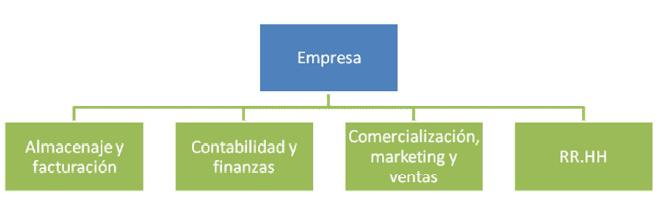
\includegraphics[keepaspectratio]{Organigrama}
	\caption{Organigrama de la empresa DIGSOL}
	\label{fig:organigrama}
\end{figure} 





\end{document}
